\section{Method}
\label{sec:method}

In order to be able to design an algorithm for diffusion limited cluster aggregation (DLCA), some familiarity to the field is required. As an introduction and preparation, the case of regulare DLA was investigated, both on and off lattice. The main interest of section \ref{sec:DLA} is just to prepare for \ref{sec:DLCA}, where a more general DLCA algorithm has been developed. However, a lot of interesting aspects that are usefull to the DLCA algorithm are uncovered.

\subsection{Diffusion limited aggregation}
\label{sec:DLA}
The fundamental algorithm of DLA, as described by Witten and Sanders \cite{PhysRevLett.47.1400} is as follows; a seed particle (the particle we follow) is placed at the centre. This particle will be the basis of the growing cluster. Another particle is then introduced at some distance from this seeding particle. The starting position of this particle can in principle be infinitely far away from the particle, but for practical matters, it is often placed close to the seeding particle. This particle will perform a random walk in the space around the seeding particle, with the intention that at some point in time, the walking particle will hit (i.e. be sufficiently close to) the seeding particle, and the two will clump together. 

All of the following algorithms have been implemented using C++ 14. \textcolor{red}{??? Don't know about the following part, but:} The code was run on OS X Yosemite 2,7 GHz Intel Core i5 8 GB 1867 MHz DDR3 system.

\subsubsection{On-lattice DLA}
\label{sec:on-lattice_method}
For the on-lattice case, the algortihm is pretty straight forward, as is described in the beginning of section \ref{sec:method}. Thus it will only briefly be discussed here, with the main focus being on the off-lattice version. Special for the on-lattice case is that the particle can only move in discrete steps and directions. That is, it may only move along the axis (either north, south, east or west), but not diagonally. More specific for the simulation run in this project is that the walking particles would always start at a random (uniformly distributed) point on the perimeter of the grid. If it was to take a step causing it to move outside of the grid, it would restart somewhere else on the perimeter. Although this cannot be done without some loss of generality, it is still done to increase the simulation speed. \textcolor{red}{??? should look into this more?}

Since the on-lattice simulation is of less interest compared to the off-lattice case, only a crude on-lattice simulation was performed. The results of the on-lattice simulations can be found in \textcolor{red}{??? Link to section with results for on-lattice DLA simulations. }

\subsubsection{Off-lattice DLA}
In off-lattice DLA simulations, the particle is no longer restricted to move along any axis. This means it can move freely in an approximately continous space, and in any direction. This necessitates a more complex algorithm than for the on-lattice case. The algorithm used for the off-lattice DLA simulation is based on the one suggested by Kuijpers et. al. \cite{Kuijpers2014841}. In this algorithm, one uses an on-lattice approximation for storing the positions of the particles in the cluster, thus being more RAM dependant than other algorithms, but with the benefit of reducing the calculation of sites viable for hits. Silimar to what was the case in section \ref{sec:on-lattice_method}, the particle starts along a circle of radius $R_{start}$ from the cluster, and will be killed if the wander too far from the cluster. This limit is set to $R_{kill} = 5R_{cluster}$, where $R_{cluster}$ is the radius of the smallest circle spanning the cluster.

\textcolor{red}{??? Write about the hit criteria! This is also used for the off-lattice DLCA program.}
As one goes from discrete to continous space, the algorithm must calculate if a hit is taking place. It is no longer enough to check if the neighbouring cell is occipied, so this is done in accordance with figure \ref{fig:L_hit}. Cartesian coordinates were used, and the exact coordinates og particles eligible for hits are extracted (see section \textcolor{red}{??? LINK TO APPROPRIATE SECTION HERE!}). As all particles are defined from their center, one has to take into account their extent (???). The distances $a$ and $b$ are found from geometric inspection of figure \ref{fig:L_hit}, giving

\begin{align}
a = x_p - (x_0 + L_{hit}\cos(\alpha)) \label{eq:a} \\
b = y_p - (y_0 + L_{hit}\sin(\alpha)).
\label{eq:b}
\end{align} 
Inserting \eqref{eq:a} and \eqref{eq:b} into $d_p^2 = a^2 + b^2$ and rearranging gives
\begin{align}
\begin{split}
d_p^2  = & L_{hit}^2 + 2\left[(x_0 - x_p)\cos(\alpha) + (y_0 - y_p)\sin(\alpha)\right]L_{hit}\\ & + \left[x_0^2 + x_p^2 + y_0^2 + y_p^2 - 2(x_0x_p + y_0y_p)\right].
\end{split}
\end{align}
This can be written on the form
\begin{align}
AL_{hit}^2 + BL_{hit} + C = 0,
\label{eq:L_hit}
\end{align}
with parameters defined by
\begin{align}
A & = 1 \\
B & = 2\left[(x_0 - x_p)\cos(\alpha) + (y_0 - y_p)\sin(\alpha)\right] \\
C & = (x_p - x_0)^2 + (y_p - y_0)^2 - d_p^2.
\end{align}

Equation \eqref{eq:L_hit} may be solved as a usual polynomial of second order, which means it may or may not have a solution. The algortihm is thus designed to take all possible situations into account. \textcolor{red}{??? May write all five cases and how the code treats them, or may just link to the Kuijpers paper?} 

\begin{figure}[h]
	\begin{center}
		\includegraphics[width = 0.4\textwidth]{fig/L_hit.png}
		\caption{Schematic of the hit calculation for off-lattice simulations. Here, the red circles are the positions of the walking particle, and the blue are particles already in the cluster. The walking particle is launched from position $x_0, y_0$ in the $\alpha$ direction with the horizontal plane. The dotted red line indicates where the walking particle would end up, if it was to take a full step of length $L_{step}$. As the walking particle will collide with the particle located in $x_p, y_p$, it cannot do the full step, but rather a smaller of length $L_{hit}$. The distance $d_p$ is the diameter of the particles, while $a$ and $b$ are geometrical distances.}
		\label{fig:L_hit}
	\end{center}
\end{figure}


With the new hit calculation routine, the concept of this new algorithm is as follows: The program uses three arrays (illustrated in figure \ref{fig:on_lattice_arrays}), which together keeps track of all information of interest. The first one, $\textbf{A}$, is an $N \times 2$ array ($N$ is number of particles), in which the exact coordinates of the particles are stored. These coordinates are then mapped to integer values, so that they may correspond to a cell number in $\textbf{B}$, an $n \times n$ ($n$ is the size of the grid used for approximations) array in which all the elements are either $0$ or the label of the particle. See figure \ref{fig:A_sketch} and \ref{fig:B_array} for an illustration of this. In this context, label refers to the number given to the particle when it attaches to the cluster. Starting from the original seed particle, which is given label 1, the particles are labeled in ascending order, meaning the first particle to hit the seed particle will get label 2 and so on. The final array, $\textbf{C}$ (also of dimension $n \times n$), stores the distance from each cell to the closest particle, as shown in figure \ref{fig:C_array}. This is done in order to have quick access to the distance from a walking particle to a point on the cluster. The great benefit of this algorithm lies in being able to take steps of varying length, depending on the distance from the cluster, which is only possible without loss of generality if the particle is far away from the cluster. There is a set a maximum distance $D_{max}$ for the distances in $\textbf{C}$, in order to reduce the amount of calculations required per time iteration. $D_{max}$ balances the length of the steps the particle may take (longer steps results in a faster program), to the number of particles needed to be checked (which slows the program down).

\begin{figure}[h]
	\begin{center}
		\begin{subfigure}[t]{0.3\textwidth}
			\includegraphics[width = \textwidth]{fig/A_sketch.png}
			\caption{Figure of the example configuration.}
			\label{fig:A_sketch}
		\end{subfigure}
		\begin{subfigure}[t]{0.3\textwidth}
			\includegraphics[width = \textwidth]{fig/B_array.png}
			\caption{How the labels of the particles would be. The original seeding particle would be numbered 1, and the other particles are labeled as they hit the cluster.}
			\label{fig:B_array}
		\end{subfigure}
		\begin{subfigure}[t]{0.3\textwidth}
			\includegraphics[width = \textwidth]{fig/C_array.png}
			\caption{Illustration of the array with the rounded off distances. Knowing what cell the walker is in, it is easy to determine its distance to the cluster.}
			\label{fig:C_array}
		\end{subfigure}
		\caption{Illustration of a dummy configuration of particles, and how each array work. The seed particle is in all cases placed in a $13 \times 13$ array, at position (7,7). For simplicity, the other particles are not random walkers in this dummy case, but move in from right to left, along the horizontal axis.}
		\label{fig:on_lattice_arrays}
	\end{center}
\end{figure}

Throughout the process, the walking particle will take steps depending on its distance from the cluster. The step direction $\alpha$ is drawn from a uniform random distribution, and is defined according to figure \ref{fig:L_hit}. The following three criterias determines the different regimes the walker may be in with respect to step size. It is worth noting that $L_{step}$ is the step size taken by the particle corresponding to Brownian motion when the particle is close to the cluster. This value is set before the simulation starts. What regime the particle is in depends on wheter the approximated distance between the walker and the cluster, $d_{wc}$, is so small that there is a chance of hitting the cluster if the particle takes a step of length $L_{step}$. The distance $d_{wc}$ can be found by looking in the cell labeled with the rounded coordinates of the walker in $\textbf{C}$. In addition, one must take into account that what is stored is the coordinates of the centre of the particles, meaning that there must be a distance of $2r_p$ between them at least. Since one looks at the rounded off coordinates in when finding $d_{wc}$, one adds a $1$ to make sure that the region includes all possibilities of hits.

\begin{itemize}
{\setlength\itemindent{1.0in}\item[$d_{wc} \le 2r_p + L_{step} + 1$:] The particle is in the short range regime, within hitting range of the cluster. That may be a single particle or lots of particles, and exact calculations are required for determining if the particle will hit any of the particles within the range of $d_{wc}$. This is done by looking at all particles stored in $\textbf{B}$ within a square of size $ 2(2r_p + L_{step} + 1)+1$ centered around the cell with indices given by the rounded coordinates of the walking particle. All non-zero elements within this square gives the location of the coordinates in $\textbf{A}$, so they can be extracted. Then the hit estimation calculations are performed for all particles within hitting range, and the one yielding the lowest positive step required will be the one the particle latches on to. 
\item[$ 2r_p + L_{step} + 1 \le  d_{wc} \le D_{max}$:] The particle is in an intermediate regime, meaning it can only move a distance of $d_{wc} - (2r_p + L_{step} + 1)$ without having to check for a possibility of a hit. 
\item[$d_{wc} = D_{max}$:] The particle is in the long range regime, far away from the cluster, allowing it to move a distance of max($d_{w0} - R_{max} - (2r_p + L_{step} + 1), D_{max} - (2r_p + L_{step} + 1)$).}
\end{itemize}

The particle will attach to the cluster iff the step performed is shorter than $L_{step}$. Then $\textbf{A}$, $\textbf{B}$ and $\textbf{C}$ are updated, and a new particle starts walking. A new walker is launched from the starting distance $R_{start}$, and this entire process is repeated until the cluster contains the desired amount of particles. At this point, the fractal dimension $d_f$ can be calculated using a fit of the data to equation \eqref{eq:N_Rg_rel}. This was done to evaluate and analyze the results.

\subsection{Diffusion limited cluster aggregation}
\label{sec:DLCA}
Diffusion limited cluster aggregation (DLCA) is the growth process where instead of starting with a seed particle and launching random walkers, one instead starts with a density of particles over a domain, and let them all do a random walk. They will similarly to the DLA case stick together on contact, causing clusters to be formed. These cluster will again move around, and attach to other clusters until all particles are part of a single cluster. 

The algortihm for DLCA has been developed for this project. It is inspired by the concepts of Kuijpers et. al. \cite{Kuijpers2014841}. However, the variable step size determination in the off-lattice DLA algorithm has not \textcolor{red}{??? YET} been implemented, as it is not as straight forward to keep track of distances between clusters and the orientation of clusters. This is partly due to the fact that all clusters will perform a random walk throughout the simulation, and may then been thought of as walkers. As with DLA, this was implemented with particles both on and off lattice. \textcolor{red}{??? To make things physical, the step length in the off-lattice simulations was calculated for each cluster according to equation \eqref{eq:diffusion_walker_relation}.}

The starting point of DLCA is to have particle density of interest, and distributes this over a domain. The particles are distributed randomly \textcolor{red}{???(uniformly at the moment)} within the given domain. For simplicity, one uses periodical boundary conditions. The hit checks/calculations are similar to those for DLA (both on and off lattice). Particle positions are stored in a dynamical array $\mathbf{\Phi}$, as seen in figure \ref{fig:clusters_schematics} and \ref{fig:clusters_example_schematic}. The labels of the clusters correspond to the column number of $\mathbf{\Phi}$, and are stored in the enumerated grid $\mathbf{\Psi}$ (see figure \ref{fig:num_grid_example}). For the off-lattice case, an extra enumerated array, $\mathbf{\Omega}$, is necessary to be able to go back and forth between the exact coordinates and mapped arrays more easily.


\begin{figure}[h]
	\begin{center}
		\includegraphics[width = 0.4\textwidth]{fig/clusters_schematics.png}
		\caption{Schematic of the structure of the $\mathbf{\Phi}$ array. Note that the dimension is not $N \times N$, but is dynamic iand will change throughout the simulation. The subscript $c$ indicates the label for the cluster, while $n$ denotes the particle number within a cluster $c$.}
		\label{fig:clusters_schematics}
	\end{center}
\end{figure}

\begin{figure}[h]
	\begin{center}
		\begin{subfigure}[t]{0.23\textwidth}
			\includegraphics[width = \textwidth]{fig/example.png}
			\caption{Example of how a configuration would look.}
			\label{fig:example}
		\end{subfigure}
		\begin{subfigure}[t]{0.23\textwidth}
			\includegraphics[width = \textwidth]{fig/num_grid_example.png}
			\caption{Example of how the $\Psi$ array would look.}
			\label{fig:num_grid_example}
		\end{subfigure}
		\begin{subfigure}[t]{0.23\textwidth}
		\includegraphics[width = \textwidth]{fig/num_grid_N_example.png}
			\caption{Example of how the $\mathbf{\Omega}$ would look. Note that this example is for on-lattice DLCA, so it is not stricly necessary, but is is uncluded for illustrational purposes.}
			\label{fig:num_grid_N_example}
		\end{subfigure}
		\begin{subfigure}[t]{0.23\textwidth}
			\includegraphics[width = \textwidth]{fig/clusters_example_schematic}
			\caption{Example of how the clusters array would look. }
			\label{fig:clusters_example_schematic}
		\end{subfigure}
		\caption{Example of how the data structures would look.}
		\label{fig:arrays}
	\end{center}
\end{figure}

This storage system allows for easy checks to see if a particle has any neighbours \textcolor{red}{(at the moment only nearest neighbours)}, which may allow for a hit. The benefit of this is that one only have to check a fraction of the total domain, limiting the computational complexity significantly. \textcolor{red}{??? This is where the hitting is explained, with the square check and everything!} More specifically, the algorithm checks a square of size $4r_p +1$ centered in the cell the particle is supposed to move to. This limits the maximum step size allowed in the program \textcolor{red}{??? calculate the limit and write about it here!}. The exact coordinates of all particles within this square is extracted, and checked for hit possibility. The one hit resulting in the shortest step performed will then be the valid one \textcolor{red}{??? rephrase}. Since the moving particle might be part of a cluster, the algorithm has to find the shortest valid step for every particle it contains before an actual move may take place.

In the event that a hit happens, the two colliding clusters will join together and form a new cluster. As a result, all arrays have to be updated, making sure the labelling of the new cluster is correct. For conventional \textcolor{red}{???consitency?} purposes, the new cluster will always have the label of the lowest numbered cluster comming in. This means if cluster 2 collides with cluster 6, the new cluster will keep label 2 while 6 is erased from $\mathbf{\Phi}$. All clusters with label higher than 6 will then have their label reduced by 1. This also means that all cells with label 6 in $\mathbf{\Psi}$ will be relabeled to 2, and all clusters with higher labels than 6 are reduced by 1. In $\mathbf{\Omega}$, there has to be a relabelling of the particles from the old cluster 6, so that they continue the labelling cluster 2 had before the collision. 

\textcolor{red}{??? Explain how when a cluster crashes into another, this will cause the cluster "crashed into" to not take a step during that time iteration. }

 After some while, one might have a situation similar to that shown in figure \ref{fig:example}. \textcolor{red}{??? elaborate on the configuration.}

When a cluster moves, all particles within the cluster moves in the same distance with the same step length. An important part of the algorithm is to keep the $\Psi$ and $\Omega$ arrays correct, even after a particle moves, as this is necessary to be able to check the correct particles for hit. \textcolor{red}{??? Write about the update process for general movement of the clusters, not related to if they hit or not. (note that this is the bug that has taken me 2 weeks to fix!)}

\textcolor{blue}{The following is what I plan to do before Dec. 18.}

\subsection{To do}

Introduce physical diffusion constant, and compare cluster size distributions to what was found in \cite{PhysRevLett.52.1669}. Then introduce a velocity field (pretty basic to begin with), and analyze the resulting distribution in the same framework. If there is time, allow for mineral dust-sized particles in the system, and allow them to "fall out". In other words, think of the figures presented here to be in the $x,y$-plane, and $z$ to be height over ground. Removing the particles will correspond to them falling down, but I will have to think about the best way to do this, while still maintaining mass conservations (introduce new small or big particles).